\newpage

\section{Initial Value Problems and Energy Estimates for the Wave Equation}

\subsection{Initial value problems for the wave equation}

Today, we will be looking at the wave equation
\begin{align*}
    &\square u = f \quad \text{in } \MM^{n+1} = \RR \times \RR^{n}\\
    & u(0) = u_0\\
    \partial_t u(0) = u_1
\end{align*}
where 
\[
    \square = \partial_t^2 -\Delta_x = - m^{\alpha \beta}\partial_\alpha \partial_\beta, \quad m=\left[\begin{array}{lllll}
        -1 & & & & \\
        & 1 & & & \\
        & & \ddots & \\
        & & & 1
        \end{array}\right].
\]
We have seen that the fundamental solution (forward in time) is
$$
K(t, x)= \begin{cases}\frac{1}{2} 1_{\{t>|x|\}} & n=1 \\ c_{n}\left(t^{2}-x^{2}\right)_{+}^{(1-n) / 2} & n \geq 2 \text { even } \\ c_{n} \delta_{t^{2}-x^{2}}^{\left(\frac{n-1}{2}\right)} & n \geq 2 \text { odd }\end{cases}
$$
The solution for the inhomogeneous problem is $u=K * f$ (as if the Cauchy data equals 0 at $-\infty)$. The solution for the homogeneous problem $\left(f=0, u_{0}, u_{1} \neq 0\right)$ is a bit more tricky. Let
$$
\tilde{u}= \begin{cases}u & t>0 \\ 0 & t<0\end{cases}
$$
Let's find an equation for $\tilde{u}$.
$$
\begin{gathered}
\Delta \widetilde{u}= \begin{cases}\Delta u & y \geq 0 \\
0 & t<0,\end{cases} \\
\partial_{t} \widetilde{u}=\left\{\begin{array}{ll}
\partial_{t} u & y>0 \\
0 & t<0,
\end{array}+\delta_{t=0} \cdot u_{0} .\right.
\end{gathered}
$$
The second time derivative is then
$$
\partial_{t} \widetilde{u}=\left\{\begin{array}{ll}
\partial_{t}^{2} u & y>0 \\
0 & t<0,
\end{array}+\delta_{t=0} \cdot u_{1}+\delta_{t=0}^{\prime} \cdot u_{0} .\right.
$$
This gives us
$$
\square \widetilde{u}=\delta_{t=0} u_{1}+\delta_{t=0}^{\prime} u_{0}
$$
which implies that
$$
\widetilde{u}=K *_{t, x}\left(\delta_{t=0} u_{1}+\delta_{t=0}^{\prime} u_{0}\right) .
$$
Taking the convolution first in $t$ gives
$$
\widetilde{u}(t)=K(t) *_{x} u_{1}+\partial_{t} K(t) *_{x} u_{0} .
$$

Here are some properties of the wave equation:
\begin{itemize}
    \item Finite speed of propagation: The solution only exists inside the positive cone. 
    \begin{figure}[H]
        \centering
        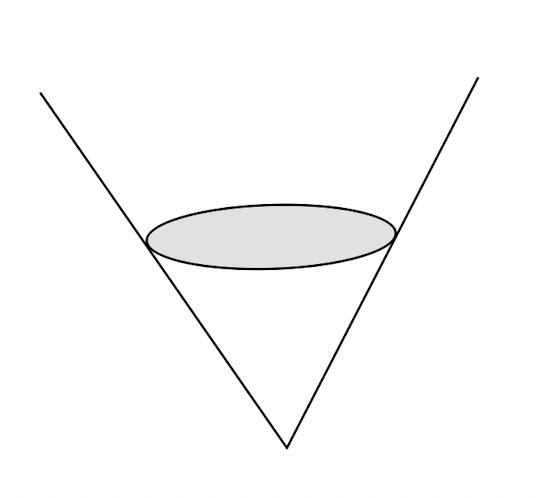
\includegraphics[width=0.4\textwidth]{pics/25-1.jpeg}
    \end{figure}
    \item Huygens principle: When $n\ge 3$ is odd, the fundamental solution is supported exactly on the cone.
\end{itemize}

Suppose now that we have some region with initial data $(u_0, u_1)$ which can be changed. Where does the solution change? At each point, we have an upward cone, and we take the union of these cones. 

\begin{figure}[H]
    \centering
    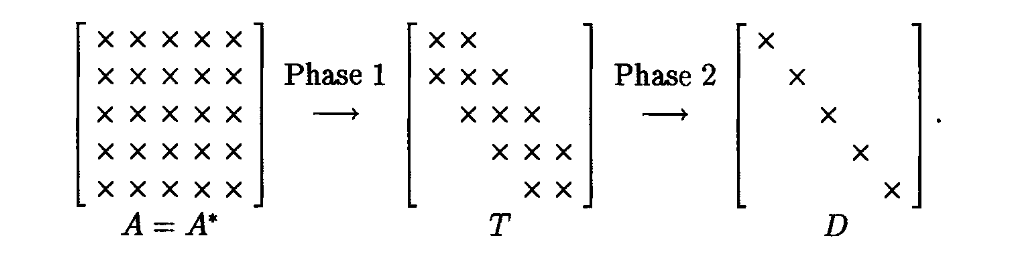
\includegraphics[width=0.7\textwidth]{Pics/25-2.png}
\end{figure}

The \textbf{domain of influence} is $\Omega=\cup_{x \in D}\{(0, x)+K\}$, where $K$ is the forward cone. Now suppose we only have initial data $\left(u_{0}, u_{1}\right)$ in the domain $D .$ Where can we find the solution? If we look at a point $(t, x)$, then $u(t, x)$ depends on $u_{0}, u_{1}$ in $B(x,|t|)$. The value $u(x, t)$ is uniquely determined if $B(x,|t|) \subseteq D$. The union, $\{(t, x): B(x,|t|) \subseteq D\}$ is called the \textbf{domain of uniqueness} for $D$.

\begin{figure}[H]
    \centering
    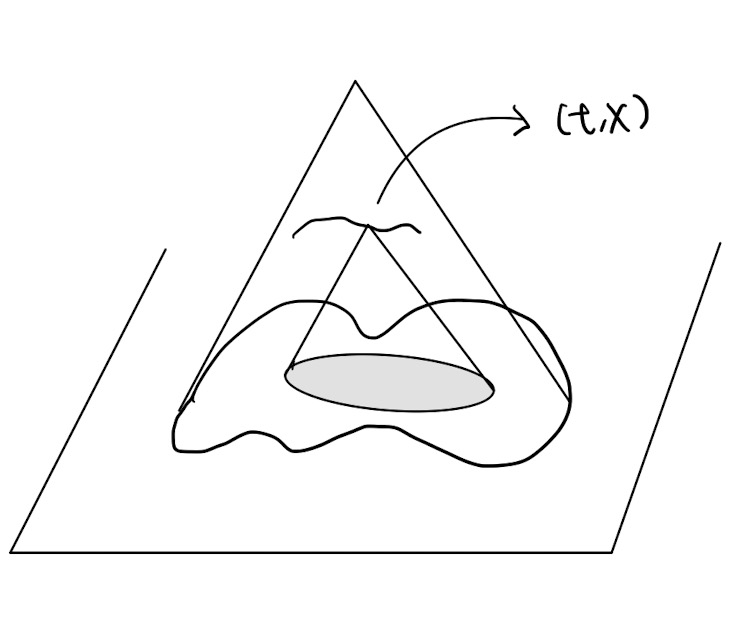
\includegraphics[width=0.5\textwidth]{Pics/25-3.png}
\end{figure}

\begin{example}
When the base domain $B$ is a ball, then the domain of uniqueness $C$ is exactly a cone:
\begin{figure}[H]
    \centering 
    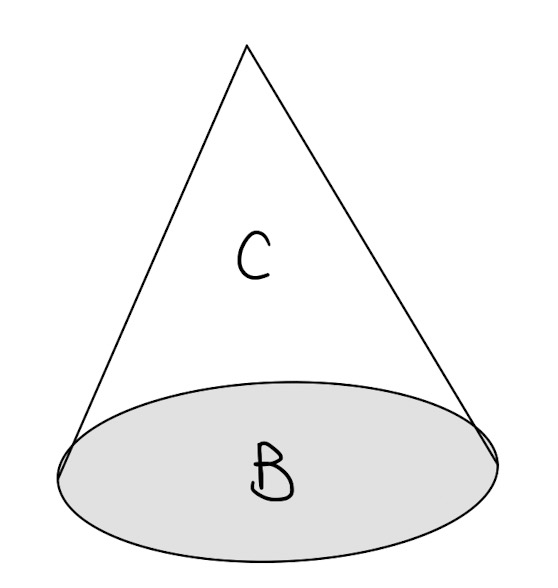
\includegraphics[width=0.3\textwidth]{Pics/25-4.png}
\end{figure}
\end{example}

\subsection{Energy estimates for the wave equation}

Here's how energy estimates work for the wave equation. When we say energy, we want to think a quantity which is conserved. Suppose we have a vibrating string.

We can 
We can think of the energy as potential energy $P$, expressed in terms of "how extended is the string." This can be measured by some average of the slope of the string:
$$
P=\int\left|\partial_{x} u\right|^{2} d x \text {. }
$$
The second part of the energy should be the kinertic energy, which measures the velocity of the string:
$$
\int\left|\partial_{t} u\right|^{2} d x
$$
If we were physicists, we would have constants in front, but we are mathematicians, so we will set some constants equal to 1. We can write the total energy as
$$
E(u(t))=\frac{1}{2} \int\left|\partial_{t} u\right|^{2}+\left|\nabla_{x} u\right|^{2} d x
$$

\begin{theorem}
    If $\square u =0$, then $E(u(t))$ is constant.
\end{theorem}

\begin{proof}
\[
    \begin{aligned}
        \frac{d}{d t} E &=\int \partial_{t} u \partial_{t}^{2} u+\sum_{j=1}^{n} \partial_{j} u \cdot \partial_{t} \partial_{j} u d x  \\
        &=\int \partial_{t} u \sum_{j=1}^{n} \partial_{j} \partial_{j} u+\sum_{j=1}^{n} \partial_{j} u \cdot \partial_{t} \partial_{j} u d x  \\
        &=0
        \end{aligned}
\]
 By Green's theorem, assuming that $ u=0 $ at $\infty$.
\end{proof}

Why should we improve on this? We have seen that "conservation laws" imply features of our problem. If we have
$$
\partial_{t} \underbrace{u}_{\text {density }}+\partial_{x} \underbrace{F(u)}_{\text {flux }}=0
$$ 

which tells us that
$$
\partial_{t} \int u \,dx=0
$$
For the wave equation, we have the energy density
$$
e(t, x)=\frac{1}{2}\left|\partial_{t} u\right|^{2}+\left|\nabla_{x} u\right|^{2},
$$
so that
$$
E=\int e
$$
Note that this doesn't go the other way around; there may be many densities that integrate to the same total energy $E$. We can look at
$$
\begin{aligned}
\partial_{t} e(t, x) &=\partial_{t} u \cdot \partial_{t}^{2} u+\partial_{j} u \cdot \partial_{t} \partial_{j} u \\
&=\partial_{t} u \cdot \square u+\partial_{t} u \cdot \partial_{j}^{2} u+\partial_{j} u \partial_{t} \partial_{j} u \\
&=\partial_{j}(\underbrace{\partial_{t} u \cdot \partial_{j} u}_{\text {energy flux }})+\partial_{t} u \cdot \square u
\end{aligned}
$$
This leads us to another proof of the energy estimates for the wave equation:

\vspace{1em}
\begin{proof}
    Start with $\square u=0$, and get $\square u \cdot \partial u=0$. Then integrate by parts.
    \qed
\end{proof}

Let's see what happens when we take
$$
\begin{aligned}
\square u \cdot \partial_{k} u &=\left(\partial_{t}^{2} u-\partial_{j} \partial_{j} u\right) \cdot \partial_{k} u \\
&=\partial_{t}\left(\partial_{t} u \cdot \partial_{k} u\right)-\partial_{t} u \cdot \partial_{t} \partial_{k} u-\partial_{j}\left(\partial_{j} u \cdot \partial_{k} u\right)+\partial_{j} u \cdot \partial_{j} \partial_{k} u
\end{aligned}
$$
We can think of the first and third terms as derivatives.
$$
=\partial_{t}(\underbrace{\partial_{t} u \cdot \partial_{k} u}_{\text {density }})-\underbrace{\frac{1}{2} \partial_{k}\left(\partial_{t} u\right)^{2}-\partial_{j}\left(\partial_{j} u \partial_{k} u\right)+\frac{1}{2} \partial_{k}\left(\partial_{j} u\right)^{2}}_{\text {divergence of a flux }}
$$
We get a new, conserved quantity, the momentum
$$
P_{k}=\int \partial_{t} u \cdot \partial_{k} u d x
$$
This tells you in what direction the energy is moving around. Conservation says that if the energy is moving around in one direction, it will be moving in that same direction forever.

More generally, consider
$\square u \cdot X u, \quad$ where $\quad X=\sum X^{\alpha} \partial_{\alpha}$
This gives a conserved quantity $E_{X}$, which is positive definite if the vector field $X$ is \textbf{forward time-like}.

\begin{figure}[H]
    \centering
    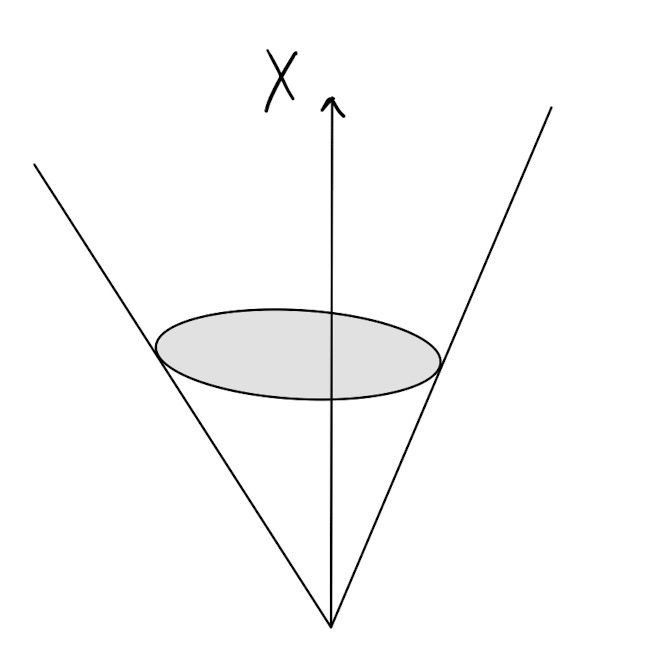
\includegraphics[width=0.3\textwidth]{pics/25-6.png}
\end{figure}

\begin{remark}
    We can put the energy and the momentum into one conserved quantity, called the energy-momentum tensor,
$$
T^{\alpha \beta}(u)=\partial^{\alpha} u \partial^{\beta} u-\frac{1}{2} m^{\alpha \beta} \partial^{\gamma} u \partial_{j} u
$$
where
$$
\partial^{\alpha}=m^{\alpha \beta} \partial_{\beta} u
$$
For the wave equation, this looks like
$$
\partial^{0} u=-\partial_{0} u, \quad \partial^{j} u=\partial_{j} u .
$$
This is a divergence free tensor:
$$
\partial_{\alpha} T^{\alpha \beta}=0 \quad \forall \beta \quad \text { if } \quad \square u=0 .
$$
If $\beta=0$, this is the energy, and if $\beta=j \neq 0$, this is the momentum $P_{j}$.
\end{remark}

\subsection{Finite speed of propagation via energy estimates}
The finite speed of propagation is a robust phenomenon. We can show this by providing a proof which does not rely on the fundamental solution and only requires energy estimates. If we have a ball $B$ for our inital data, and a cone $C$, we want to show that $\left(u_{0}, u_{1}\right)$ in $B$ uniquely determines the solution in $C$.

\begin{figure}[H]
    \centering
    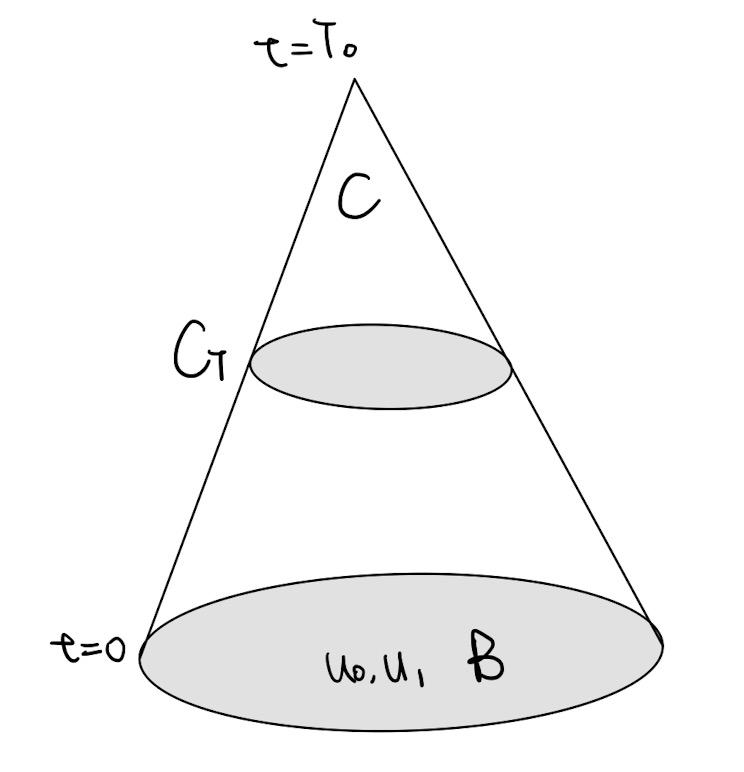
\includegraphics[width=0.3\textwidth]{Pics/25-7.png}
\end{figure}
This is the same as saying that if $\left(u_{0}, u_{1}\right)=(0,0)$ in $B$, then $u=0$ in $C .$ Suppose we want to show that $u=0$ in the slice $C_{T}$ of the cone. We saw the following density flux relation for the energy:
$$
\partial_{t} e(t, x)=\partial\left(\partial_{t} u \cdot \partial_{u}\right)
$$
Integrate over $C_{[0, T]}$, the section of the cone up to time $T$.
$$
\int_{C_{T}} e-\int_{C_{0}} +\int_{\partial C_{[0, T]}} e \cdot \nu_{t}-p_{j} \nu_{x}=0
$$
Moving the middle term to the right hand side, this tells us that
$$
\operatorname{Energy}(t=0)=\operatorname{Energy}(t=T)+\text { Flux (boundary) }
$$
The former term is the part that is left in the cone, and the latter term is the part that goes out. If the energy at time $t=0$ is 0, then these two terms must both equal $0 .$

The remaining objective is to show that the Flux term is nonnegative. What does it mean that the slope of the cone is $-1$ ? This means that the outward pointing normal is $\nu=(1, \omega)$ with $|\omega|=1$. Then
$$
\begin{aligned}
e \cdot \nu_{t}-p_{j} \cdot \nu_{j} &=\frac{1}{2}\left(u_{t}^{2}+\left|\nabla_{x} u\right|^{2}\right)-\partial_{t} u \cdot \partial_{j} \cdot \omega_{j} \\
& \stackrel{?}{\geq} 0
\end{aligned}
$$
We can use Cauchy-Schwarz twice to say
$$
\begin{aligned}
\left|\partial_{t} u \cdot \partial_{j} u \cdot \omega_{j}\right| & \leq\left|\partial_{t} u\right| \cdot|\partial u| \\
& \leq \frac{1}{2}\left(\left|\partial_{t} u\right|^{2}+|\partial u|^{2}\right)
\end{aligned}
$$